\documentclass[11pt, a4paper]{amsart}
\usepackage{parskip} 
\usepackage{pgfplots}
\usepackage{graphicx}
\title{MAS116/117: Lab 4 Experiments}
\author{Nur Farhazni Najwa Binti Farhan}

\begin{document} 
\maketitle
\section{Graphs created with PGFplots}

\begin{center} %center the graph
\begin{tikzpicture} %will produce normal graph
	\begin{axis}[
		axis lines=center, %the box disappear
		title={$y=\sin (deg(x))$}, %deg(x) function takes a number (in radians) and turns it into the value in degrees; that is, deg(x) = 180x/π
		xlabel=$x$, ylabel=$y$]
	\addplot[smooth, domain=-2*pi:2*pi]{sin(x)};
	\end{axis}
\end{tikzpicture}

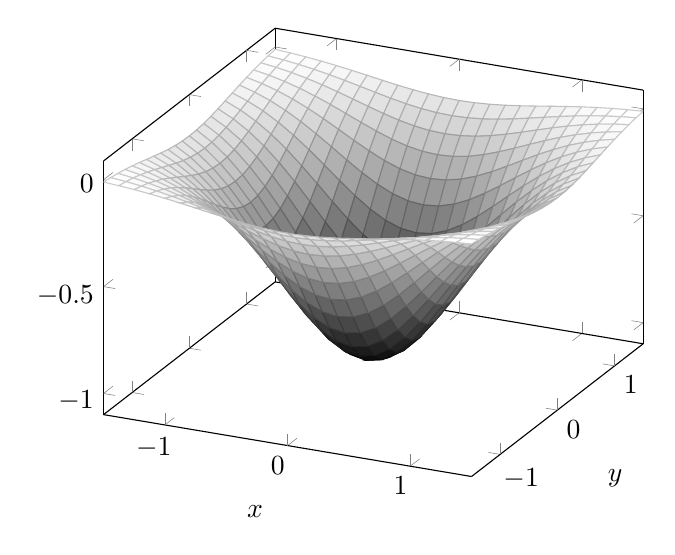
\begin{tikzpicture} %will produce 3d graph
	\begin{axis}[xlabel=$x$, ylabel=$y$, colormap/blackwhite] %put comma, and colormap will produce image in bw
		\addplot3[domain=-1.5:1.5, surf]{-exp(-x^2 - y^2)};
	\end{axis}
\end{tikzpicture}
\end{center}
%more graph : http://pgfplots.sourceforge.net/gallery.html. 

\section{Including image files}
\includegraphics{geogebra_image.pdf}
\end{document} 
